\addcontentsline{toc}{chapter}{Занятие 1. Элементы комбинаторики}
\chapter*{Занятие 1. Элементы комбинаторики}

\addcontentsline{toc}{section}{Контрольные вопросы и задания}
\section*{Контрольные вопросы и задания}

\subsubsection*{Сформулируйте основной принцип комбинаторики (правило умножения).}

Если множества
$A_1,  \dotsc , A_m$
содержат соответственно $n_1,  \dotsc , n_m$
элементов, то количество m-мерных векторов, которые получают выбором по одному элементу из каждого множества равно
$n_1\cdot n_2\cdot \dotsc \cdot n_m$.

\subsubsection*{Что называется сочетанием из n элементов по k?}

В комбинаторике сочетанием из n по k называется набор k элементов, выбранных из данного множества, содержащего n различных элементов.

\subsubsection*{Чему равно число сочетаний из n элементов по k?}

Если некоторое множество содержит n элементов, то количество её k-элементных подмножеств равно
$$ C_n^k = C_n^{n-k} = \frac{n!}{k!\left(n-k\right)! = \frac{n\cdot\left(n-1\right) \cdot \dotsc \cdot \left( n-k+1 \right) }{k!}} , $$
где $n!=1\cdot 2\cdot \dotsc \cdot n$.
Считается, что $0!=1$.

\subsubsection*{Что называется сочетанием с повторениями из n элементов по k?}

Сочетанием (комбинацией) с повторениями называется набор из n элементов, каждый из которых может быть одного из k типов.

\subsubsection*{Чему равно число сочетаний с повторениями из n элементов по k?}

Количество разных комбинаций из элементов n типов по k с повторениями равно
$$C_n^k=C_{n+m-1}^{m-1}=C_{n+m-1}^n.$$

\subsubsection*{Что называется размещением из n элементов по k?}

Размещения из n элементов по k --- это упорядоченные k-элементные подмножества множества, которое состоит из n элементов.

\subsubsection*{Чему равно число размещений из n элементов по k?}

Количество размещений из n элементов по k равно
$$A_n^k=k!C_n^k=n\cdot(n-1)\cdot \dotsc \cdot(n-k+1).$$

\subsubsection*{Чему равно число перестановок множества из n элементов?}

Количество перестановок равно $n!$.

\subsubsection*{Чему равно число способов разбиения множества из n элементов на m непересекающихся неупорядоченных подмножеств, которые содержат соответственно $k_1,  \dotsc , k_m$ элементов?}

Первое подмножество содержит $k_1$ элемент.
Количество комбинаций, которыми можно выбрать эти элементы, равно $C_n^{k_1}$.
Второе подмножество содержит $k_2$ элементов, тогда его элементы можно выбрать $C_{n-k_1}^{k_2}$ способами.
Подмножество под номером m содержит $k_m$ элементов.
Эти элементы можно выбрать из оставшихся
$ \left( n - k_1 - k_2 - \dotsc - k_{m-1} \right) $
$C_{n-k_1-k_2- \dotsc - k_{m-1} }^{k_m} $ способами.
Число способов разбиения множества из n элементов на m непересекающихся неупорядоченных подмножеств равно
$$ C_n^{k_1} \cdot C_{n-k_1}^{k_2} \cdot \dotsc \cdot C_{n-k_1-k_2 - \dotsc - k_{m - 1} }^{k_m} = \prod \limits_{i=1}^m C_{n-\sum \limits_{j=0}^{i-1} k_j}^{k_i}.$$
Так как $$ n = k_1 + k_2 + \dotsc + k_m = \sum \limits_{i=1}^m k_i = K_i,$$
то произведение можно записать в виде
$$ \prod \limits_{i=1}^m C_{K_i}^{k_i}.$$

\addcontentsline{toc}{section}{Аудиторные задачи}
\section*{Аудиторные задачи}

\subsubsection*{1.3}

\textit{Задание.} Посетителям кафе в качестве первого блюда предлагают борщ или суп, в качестве основного блюда --- мясо, рыбу или вегетарианский салат, в качестве десерта --- мороженое или пирожное.
Подсчитать, сколько разных обедов из трёх блюд можно заказать в этом кафе.

\textit{Решение.} Есть два варианта выбора первого блюда: борщ и суп.
Число способов выбрать первое блюдо равно $C_2^1=2$.
Основное блюдо можно выбрать тремя, т.е. $C_3^1$ способами, так как есть 3 разных блюда на выбор.
На десерт предлагают два блюда на выбор, поэтому есть $C_2^1=2$ способа его заказать.
Отсюда имеем, что из указанных блюд можно заказать
$$ C_2^1 \cdot C_3^1 \cdot C_2^1 = 2 \cdot 3 \cdot 2 = 12 $$ обедов.

\subsubsection*{1.4}

\textit{Задание.} Репертуар оркестра состоит из тридцати симфоний Гайдна, девяти симфоний Бетховена и четырёх концертов Моцарта.
На концерте оркестр должен исполнить три произведения.
Подсчитать количество способов составить концертную программу, если:
\begin{enumerate}[label=\alph*)]
\item сначала необходимо исполнить произведение Гайдна, потом --- Бетховена и к завершению --- Моцарта;
\item в программу должно войти по одному произведению Гайдна, Бетховена и Моцарта, исполнять которые можно в произвольном порядке;
\item в программу должны войти три произвольные произведения из репертуара оркестра и выполнять их можно в произвольном порядке.
\end{enumerate}

\textit{Решение.} 

\begin{enumerate}[label=\alph*)]
\item Первым произведением должно быть произведение Гайдна.
Таких в репертуаре оркестра есть тридцать.
Одно произведение из тридцати можно выбрать $C_{30}^1=30$ способами.
Вторым произведением должна быть симфония Бетховена.
Количество способов выбрать одну симфонию из десяти равно $C_9^1=9$.
Из четырёх концертов Моцарта один можно выбрать $C_4^1=4$ способами.
Итого $$C_{30}^1\cdot C_9^1\cdot C_4^1=30\cdot 9\cdot 4$$ способа составить концертную программу.

\item Так как порядок исполнения произведений не важен, то на на любом из трёх мест может быть произведение любого из указанных авторов.
Отсюда имеем, что результат, полученный в пункте а) нужно умножить на $3!$.
Тогда количество способов составить концертную программу, где будет звучать по одному произведению каждого исполнителя, равно
$$ 3! \cdot C_{30}^1 \cdot C_9^1 \cdot C_4^1 = 3! \cdot 30 \cdot 9 \cdot 4.$$

\item На первом месте в концертной программе может стоять любое произведение из $30+9+4=43$ возможных.
Количество способов его выбрать равно $C_{43}^1=43$.
На втором месте --- любое из 42 оставшихся.
Это $C_{42}^1=42$.
На третьем --- любое из оставшихся 41 произведения.
Есть $C_{41}^1=41$ способ, чтобы его выбрать.
Отсюда имеем, что составить концертную программу можно
$$ C_{43}^1 \cdot C_{42}^1 \cdot C_{41}^1 = 43 \cdot 42 \cdot 41 $$ способом.
\end{enumerate}

\subsubsection*{1.5}

\textit{Задание.} В цифровом компьютере один бит --- это одно из чисел $\{0, 1\}$, а слово --- это произвольная строка из 32-х бит.
Подсчитать количество разных слов.

\textit{Решение.} В данном случае имеем множество, которое содержит 32 бита двух типов.
В качестве первого символа 32-битного слова можно выбрать одно из двух чисел.
Количество способов это сделать равно $C_{2}^1=2$.
Аналогично на всех остальных позициях может стоять либо 0, либо 1.
Отсюда имеем, что всего можно составить $2^{32}$ слова.

\subsubsection*{1.6}
\textit{Задание.} Сколькими способами можно упорядочить множество $\{1, 2,  \dotsc , 2n\}$ так, чтобы каждое чётное число имело чётный номер?

\textit{Решение.} Каждое чётное число должно стоять на чётной позиции, каждое нечётное число --- на нечётной.
В множестве есть n чётных и n нечётных чисел.
Количество способов разместить n чётных чисел на n чётных позициях равно $n!$.
Аналогично можно разместить n нечётных чисел на n нечётных позициях $n!$ способами.
Так как независимо заполняем n и n ячеек, то множество можно упорядочить $n!\cdot n!$ способами.

\subsubsection*{1.7}

\textit{Задание.} Среди 11-ти преподавателей кафедры есть 6 мужчин и 5 женщин.
Сколькими способами из них можно выбрать комиссию из 3-х человек так, чтобы в ней было 2 мужчины и одна женщина?

\textit{Решение.} Двух мужчин из шести можно выбрать $C_6^2$ способами. 
Одну женщину из пяти --- $C_5^1$ способами.
Тогда комиссию можно выбрать $C_6^2\cdot C_5^1$ способами.

\subsubsection*{1.8}

\textit{Задание.} Сколькими способами можно разместить 15 томов на книжной полке так, чтобы том I и II не стояли рядом?

\textit{Решение.} Определим общее число перестановок из 15 элементов по формуле $P_{15}=15!$.

Чтобы вычислить число <<лишних>> перестановок, сначала определим, сколько вариантов, в которых 2-й том находится рядом с 1-ым справа от него.
В таких перестановках 1-ый том может занимать места с первого по 14-е, а второй со второго по 15-е --- всего 14 мест для этой пары книг.
И при каждом таком положении первых двух томов остальные 13 книг могут занимать остальные 13 мест в произвольном порядке.
Вариантов перестановки 13 книг $P_{13}=13!$.
Всего лишних вариантов 2-го тома справа от 1-го получится $14\cdot 13!=14!$.

Аналогично рассмотрим случай, когда второй том расположен рядом с 1-ым, но слева от него.
Получается такое же число вариантов $14\cdot 13!=14!$.

Значит всего <<лишних>> перестановок $2\cdot 14!$, а нужных способов расстановки $15!-2\cdot 14!$.

\subsubsection*{1.9}

\textit{Задание.} Сколькими способами можно распределить 12 разных предметов между тремя людьми так, чтобы каждый получил 4 предмета?

\textit{Решение.} Первый человек может получить любые 4 предмета из 12.
Способов это сделать $C_{12}^4$.
Второй человек может выбрать любые 4 предмета из 8 оставшихся --- это $C_8^4$.
Третьему человеку число способов дать 4 предмета равно $C_4^4$.
Отсюда имеем, что распределить предметы можно $C_{12}^4\cdot C_8^4\cdot C_4^4$ способами.

\subsubsection*{1.10}

\textit{Задание.} Сколькими способами можно распределить 3 ириски, 5 карамелек и 12 шоколадных конфет среди 20-ти детей так, чтобы:
\begin{enumerate}[label=\alph*)]
\item каждый ребёнок получил по конфете?
\item каждый ребёнок мог получить произвольное количество конфет?
\end{enumerate}

\textit{Решение.}
\begin{enumerate}[label=\alph*)]
\item В данном случае имеем множество, которое содержит 20 конфет 3 типов, причём ириски встречаются 3 раза, карамельки --- 5 раз, а шоколадные конфеты --- 12 раз.

Допустим, нужно распределить среди детей $3+5+12$ разных конфет.
Есть $\left(3+5+12\right)!$ способов это сделать.
А теперь нужно учесть, что из них 3 одинаковые, и не брать во внимание перестановки между ними ---
$$ \frac{ \left( 3 + 5 + 12 \right)!}{3!}.$$
Но 5 и 12 из них тоже одинаковые.
Тогда количество разных перестановок равно
$$ C_{20} \left( 3, 5, 12 \right) = \frac{20!}{3!5!12!}.$$

\item Данная задача является интерпретацией задачи о заполнении перенумерованных урн шариками.
Роль урны --- ребёнок, количества шариков, которые попали в урну --- количество конфет, которые достались ребёнку.

Обозначим через $k_i$ количество конфет, которые получил $i$-й ребёнок, причём $0 \leq k_i \leq 20, \, k_1 + k_2 + \dotsc + k_{20} = \sum \limits_{i=1}^{20} k_i = 20$.

Изобразим задачу на рисунке \ref{fig:110}.

\begin{figure}[h!]
  \centering
  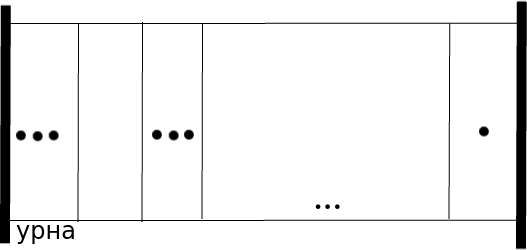
\includegraphics[width=.4\textwidth]{./pictures/1_10.png}
  \caption{Заполнение урн}
  \label{fig:110}
\end{figure}
\end{enumerate}

Урна находится между двумя палочками.
В одной урне может быть от $k_i$ шариков.
Точками обознычены шарики.
На данном рисунке в первой и третьей урнах находится по 3 шарика, во второй --- ни одного, в последней --- 1.

Палочек есть 19, а точечек (это конфеты) --- 20.
Их должны расставить на $19 + 20$ мест произвольным образом.
Количество этих решений является таким:
$$C_{20+20-1}^{19} \cdot C_{20}^{20} =
C_{39}^{19} =
\frac{39!}{19!20!} =
68923264410.$$

\subsubsection*{1.11}

\textit{Задание.} Вычислить количество неубывающих путей на двумерной целочисленной решётке
$$ \mathbb{Z}_+^2 = \{ \left( i, j \right): i, j = 0, 1, 2,  \dotsc \},$$
которые начинаются в точке $ \left( 0, 0 \right) $ и приводят в точку $ \left( m, n \right) $.
(Путь считается неубывающим, если на каждом шаге изменяется только одна координата, увеличиваясь на единицу.)

\textit{Решение.} Имеем пути, состоящие из $m+n$ ходов, среди которых ровно m <<горизонтальных>> и n <<вертикальных>> ходов.
Если выберем, на каких шагах увеличиваем одну координату (например, вертикальную), будем однозначно знать, где увеличиваем вторую координату (идём по горизонтали).
Значит, достаточно расставить m одинаковых шагов вверх на $n+m$ разных ячеек.
Это будет $$ C_{n+m}^m = \frac{ \left( n+m \right)!}{n!m!}.$$

\subsubsection*{1.12}

\textit{Задание.} Вычислить количество разных частных производных порядка r бесконечно дифференцируемой функции n переменных $f\left(x_1,  \dotsc , x_n\right)$.

\textit{Решение.} Функция бесконечно дифференцируема, значит, производная порядка r есть.
Рассмотрим функцию $f(x, y)$.
Производные первого порядка: $f'_x, f'_y$.
Первая производная --- одномерная матрица (вектор).
Производные второго порядка для
$f(x, y)$: $f''_{xx}, f''_{xy}, f''_{yx}, f''_{yy}$. $f''_{xy}$ и $f''_{yx}$
одинаковые.
Представим вторую производную в виде матрицы:
$$
\begin{pmatrix}
  xx & yx \\
  xy & yy \\ 
\end{pmatrix}
$$

Если три переменные:
$$
\begin{pmatrix}
  xx & yx & zx \\
  xy & yy & zy \\
  xz & yz & zz \\ 
\end{pmatrix}
$$

Строим матрицы по определённому алгоритму.
Столбцы --- это первое измерение, а строки --- второе.
Столбцы соответствуют x, y и z, и в ячейках столбцов на первой позиции стоит соответствующий дифференциал.
В ячейках строк указано, какой дифференциал будет вторым.

Рассмотрим третью производную для функции трёх переменных --- это трёхмерная матрица.
Третье измерение показывает, какой дифференциал будет третьим.
Значит, срез --- это то, где третьи дифференциалы фиксированы.
Получится три обычные матрицы: в первой на третьей позиции будут x, во второй --- y, а в третьей --- z.
Имеем: 
$$
\begin{pmatrix}
xxx & yxx & zxx \\ 
xyx & yyx & zyx \\
xzx & yzx & zzx \\
\end{pmatrix}
,
\begin{pmatrix}
xxy & yxy & zxy \\
xyy & yyy & zyy \\
xzy & yzy & zzy \\
\end{pmatrix}
,
\begin{pmatrix}
xxz & yxz & zxz \\
xyz & yyz & zyz \\
xzz & yzz & zzz \\
\end{pmatrix}
.$$

Матрицы записаны с учётом повторения элементов, значит нужно взять только те элементы, которые лежат на диагонали и с одной стороны от неё (треугольник).
Задача сведена к подсчёту количества элементов в r-мерной матрице $n\times n$.

Производный первого порядка есть столько же, сколько переменных у функции, т.е. n.

Найдём количество элементов двумерной матрицы $n\times n$, её верхнего треугольника.
Всего элементов в матрице $n\cdot n=n^2$.
Возьмём половину: $$\frac{n\cdot n}{2}$$ и прибавим ещё половину диагонали, чтобы получить треугольник, получаем
$$ \frac{n \cdot n}{2} + \frac{n}{2} = \frac{n(n+1)}{2}.$$

Для трёхмерной матрицы $n\times n$ проделываем аналогичные шаги.
Всего есть $n \cdot n \cdot n = n^3$ элементов, на диагонали --- $n \cdot n = n^2$ элементов.
Имеем: $$ \frac{n \cdot n \cdot n}{2} + \frac{n \cdot n}{2} = \frac{n^2(n+1)}{2}.$$

Обобщим для r-мерной матрицы.
Всего элементов $n^r$, элементов на диагонали $n^{r-1}$.
Отсюда имеем, что элементов на диагонали и выше её
$$ \frac{n^r}{2} + \frac{n^{r-1}}{2} = \frac{n^{r-1}(n+1)}{2}.$$

Это и есть число разных частных производных функции n переменных порядка r.

\subsubsection*{1.13}

\textit{Задание.} Пусть $\omega_m$ --- количество таких перестановок элементов множества $\{1, 2,  \dotsc , n\}$, что ни одно из чисел не остаётся на своём месте.
Доказать, что величина $ p_n = \frac{\omega_n}{n!}$ равна
$$ p_n = \frac{1}{2!} - \frac{1}{3!} + \dotsc + \frac{\left(-1\right)^n}{n!}.$$

\textit{Решение.} Найдём значение величины $\omega_n$.

Любая перестановка $k_1k_2 \dotsc k_n$ чисел $1, 2,  \dotsc , n$ означает вариант перестановки чисел, при котором i-е число стоит на $k_i$-м месте.
Например, в случае четырёх чисел перестановка 3241 означает,
что на первом месте стоит тройка $ \left( k_1 = 3 \right) $,
на втором --- двойка (на своём месте, $k_2=2$), на третьем --- четвёртая $ \left( k_3 = 4 \right) $ и на последнем --- первая $ \left( k_4 = 1 \right) $.
Наоборот, каждый вариант перестановки чисел обозначается единственной перестановкой чисел $1, 2,  \dotsc , n$.

Будем говорить, что в перестановки
$ k_1 k_2 \dotsc k_n $ чисел $1, 2,  \dotsc , n$
число i стоит на своём месте, если $ k_i = i $ (например, в перестановке 3241 двойка стоит на своём месте).
Нас интересует количество беспорядков, то есть таких перестановок, в которых ни одно из чисел не стоит на своём месте.
Число беспорядков можно найти, вычитая из общего количества перестановок, равного $n!$, количество тех перестановок, в которых хотя бы одно из чисел стоит на своём месте.

Пусть $A_i$ --- множество перестановок, в которых число i стоит на своём месте $\left(i=1, 2,  \dotsc , n\right)$.
Искомое число $\omega_n$ беспорядков, таким образом, равно
\begin{equation*}
\begin{split}
\omega_n =
n! - |A_1 \cup A_2 \cup \dotsc \cup A_n| = n! - \sum \limits_i |A_i| + \sum \limits_{i<j} |A_i \cap A_j| - \\
-\sum \limits_{i<j<k} |A_i \cap A_j \cap A_k| + \dotsc + \left( -1 \right)^n |A_1 \cap A_2 \cap \dotsc \cap A_n|.
\end{split}
\end{equation*}

$ |A_i| = \left( n-1 \right)!$, поэтому
$$ \sum \limits_i |A_i| = n \cdot \left( n-1 \right)! = n!.$$

Так же $ |A_i \cap A_j| = \left( n-2 \right)!$ и
$$ \sum \limits_{i<j} |A_i \cap A_j| = C_n^2 \cdot \left( n-2 \right)! = \frac{n \left( n-1 \right)}{2!} \cdot \left( n-2 \right)! = \frac{n!}{2!}.$$

Аналогично $ |A_i \cap A_j \cap A_k| = \left( n-3 \right)!$ и
$$ \sum \limits_{i<j<k} |A_i \cap A_j \cap A_k| =
C_n^3 \cdot \left( n-3 \right)! =
\frac{n \left( n-1 \right) \left( n-3 \right) }{3!} \cdot \left( n-3 \right)! =
\frac{n!}{3!}.$$

Теперь приходим к нужной формуле:
$$ \omega_n =
n! - n! + \frac{n!}{2!} =
\frac{n!}{3!} + \dotsc + \left( -1 \right)^n =
n! \cdot \sum \limits_{k=0}^n \frac{ \left( -1 \right)^k }{k!}.$$

Так как числа переставляются случайным образом, то вероятность беспорядка равна
$$ p_n =
\frac{ \omega_n }{n!} =
\frac{1}{n!} \left( \frac{n!}{2!} - \frac{n!}{3!} + \dotsc + \left( -1 \right)^n \right) =
\frac{1}{2!} - \frac{1}{3!} + \dotsc + \frac{ \left( -1 \right)^n}{n!}.$$

\subsubsection*{1.14}

\textit{Задание.} В классе учится 35 учеников.
Из них 20 занимаются в математическом кружке, 11 --- в физическом, а 10 учеников не посещают ни одного кружка.
Сколько учеников посещают математический и физический кружок.
Сколько учеников посещают только математический кружок?

\textit{Решение.} Изобразим диаграмму Эйлера-Венна для данной задачи на рисунке \ref{fig:114}. 

\begin{figure}[h!]
  \centering
  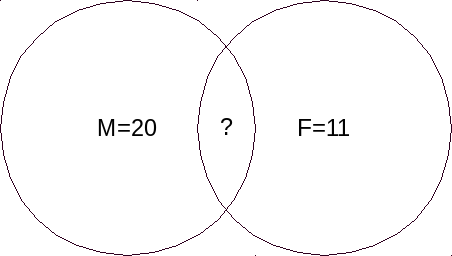
\includegraphics[width=.4\textwidth]{./pictures/1_14.png}
  \caption{Диаграмма Эйлера-Венна для задачи 1.14}
  \label{fig:114}
\end{figure}

Найдём, сколько учеников занимается хотя бы в одном кружке.
Это будет $35-10=25$ учеников.
Это есть количество элементов объединения двух множеств:
$$ |M \cup F| =
|M| + |F| - |M \cap F| =
25.$$
Отсюда можем найти, сколько учеников посещают и математический, и физический кружки:
$$ |M \cap F| =
|M| + |F| - |M \cup F| =
20 + 11 - 25 = 6.$$
Только математический кружок посещает $ |M| - |M \cap F| = 20 - 6 = 14$ учеников.

\addcontentsline{toc}{section}{Дополнительные задачи}
\section*{Дополнительные задачи}

\subsubsection*{1.15}

\textit{Задание.} Пусть множество X содержит n элементов, а множество Y --- m элементов.
Вычислить:
\begin{enumerate}[label=\alph*)]
\item количество функций из X в Y;
\item количество инъекций из X в Y $\left(n\leq m\right)$;
\item количество биекций из X в Y $\left(n=m\right)$.
\end{enumerate}

\textit{Решение.}
\begin{enumerate}[label=\alph*)]
\item Можно считать, что $ X = \{1,  \dotsc , n \}, Y = \{1,  \dotsc , m \}$.
Каждую функцию можно отождествлять с последовательностью $ < f(1),  \dotsc , f(n) ) > = < y_1,  \dotsc , y_n > $.
Каждый член $y_i$ последовательности можно выбрать m способами, что даёт $m^n$ возможностей выбора $ < y_1,  \dotsc , y_n > $.

\item Будем определять число инъективных (то есть имеющих все различные члены) последовательностей $ < y_1,  \dotsc , y_n > $.
Элемент $y_1$ может быть выбран m способами, элемент $y_2$ можно выбрать $m-1$ способом из оставшихся элементов.
Если уже выбраны элементы $ y_1,  \dotsc , y_{i-1} $,
то в качестве $y_i$ может быть выбран любой из $m-i+1$ элементов множества
$Y\setminus\{y_1,  \dotsc , y_{i-1}\}$. Принимаем, что $ m \geq n $. если $ n > m $,
то искомое число функций равно 0.
Это даёт
$$m\left(m-1\right) \dotsc (m+n-1)
=\frac{m!}{\left(m-n\right)!}$$
возможность выбора инъективных последовательностей $<y_1,  \dotsc , y_n>$.

\item Если $n=m$, то любое инъективное отображение будет биективным.
Число всех биективных отражений X в Y равно $n!$ при $m = n$ и 0 при $m \neq n$.
\end{enumerate}

\addcontentsline{toc}{section}{Домашнее задание}
\section*{Домашнее задание}

\subsubsection*{1.16}

\textit{Задание.} Подсчитать, сколько трёхзначных чисел можно записать с помощью:
\begin{enumerate}[label=\alph*)]
\item цифр 0, 1, 2, 3, 4, 5;
\item цифр 0, 1, 2, 3, 4, 5, если каждую из цифр использовать не больше одного раза.
\end{enumerate}

\textit{Решение.} Трёхзначное число можно рассматривать как трёхмерный вектор.
Первой компонентой этого вектора может быть любая цифра из множества
$$ A_1 = \{ 1, 2, 3, 4, 5 \} $$
(запись числа не может начинаться с 0).

\begin{enumerate}[label=\alph*)]
\item На остальных позициях может стоять любая цифра, то есть
$$ A_i = \{ 0, 1, 2, 3, 4, 5 \}, i = 2, 3.$$
Отсюда имеем, что из указанных цифр можно составить $ 5 \cdot 6 \cdot 6 = 180$ трёхзначных чисел.

\item На остальных позициях могут стоять любые цифры (кроме тех, что стояли на предыдущих позициях).
Отсюда имеем, что из указанных цифр можно составить $ 5 \cdot 5 \cdot 4 = 100 $ трёхзначных чисел.
\end{enumerate}

\subsubsection*{1.17}

\textit{Задание.} Подсчитать количество пятизначных чисел, которые делятся на 5.

\textit{Решение.} Пятизначное число можно рассматривать как пятимерный вектор.
Первой компонентой этого вектора может быть любая цифра из множества
$$ A_1 = \{ 1, 2, 3, 4, 5, 6, 7, 8, 9 \} $$
(запись числа не может начинаться с 0), а на остальных позициях (кроме последней) может стоять любая цифра, то есть
$$ A_i = \{ 0, 1, 2, 3, 4, 5, 6, 7, 8, 9 \}, i = 2, 3, 4.$$
На последней позиции может стоять цифра из множества $ A_5 = \{ 0, 5 \}$ (чтобы число делилось на 5, оно должно оканчиваться на 0 или 5).
Отсюда имеем, что можно составить $ 9 \cdot 10 \cdot 10 \cdot 10 \cdot 2 = 18000$ пятизначных чисел, которые делятся на 5.

\subsubsection*{1.18}

\textit{Задание.} Замок компьютерного центра состоит из пяти кнопок, пронумерованных от 1 до 5.
Чтобы открыть замок, необходимо первые две определённые кнопки нажать одновременно, а потом одну за другой нажать другие три кнопки в определённой последовательности. Подсчитать количество способов закодировать вход в компьютерный центр.

\textit{Решение.} Рассмотрим 3 случая: 
\begin{enumerate}[label=\alph*)]
\item сначала необходимо нажать две разные кнопки, далее их отпускают, и все остальные кнопки могут быть любыми; 
\item первые две кнопки держатся нажатыми, следующие кнопки не могут быть такими, как первые две; 
\item нельзя нажать одну и ту же кнопку больше одного раза (кнопки остаются нажатыми).
\end{enumerate}

Количество способов нажать первые две кнопки равна количеству двухэлементных подмножеств в множестве из пяти элементов, то есть
$$ C_5^2 = \frac{5!}{2! \left( 5 - 2 \right)!} = 10.$$

В случае а) количество способов закодировать вход в компьютерный центр равно
$$ C_5^2 \cdot 5^3 = 1250.$$
Общая формула: $ C_N^n \cdot N^m $, где N --- количество кнопок, n кнопок нажимаются вместе, а затем m кнопок --- по очереди.

В случае б) после нажатия двух кнопок, остаётся только 3 кнопки, которые необходимо нажать в правильном порядке,
поэтому количество способов по предыдущей формуле равно
$$ C_5^2 \cdot 3^3 = 270.$$

В случае в) все кнопки должны быть нажаты один раз, поэтому количество способов закодировать вход равно
$$ C_5^2 \cdot 3 \cdot 2 \cdot 1 = 60.$$

\subsubsection*{1.19}

\textit{Задание.} Колоду игральных карт (52 карты, 4 масти по 13 карт в каждой) тщательно перетасовали.
Подсчитать количество способов выбрать из неё 6 карт без возвращения так, чтобы среди них:
\begin{enumerate}[label=\alph*)]
\item был пиковый король;
\item были представители всех мастей;
\item было ровно 5 карт одной масти.
\end{enumerate}

\textit{Решение.}
\begin{enumerate}[label=\alph*)]
\item Выбрать пикового короля есть только один способ.
Остальные 6 карт могут быть любыми из оставшихся 51 карты.
Выбрать эти 5 карт можно $ C_{51}^5 $ способами.
Отсюда имеем, что из колоды можно выбрать 6 карт, среди которых был бы пиковый король, $ 1 \cdot C_{51}^5 $ числом способов.

\item Сначала выберем по одной карте каждой масти.
Количество способов выбрать одну карту определённой масти равно $C_{13}^1$, так как имеется 13 карт каждой масти.
Так как всего есть 4 масти, то нужно выбрать 4 карты (по одной карте каждой масти).
Тогда количество способов выбрать 4 карты разных мастей равно
$$ C_{13}^1 \cdot C_{13}^1 \cdot C_{13}^1 \cdot C_{13}^1 =
\left( C_{13}^1 \right)^4.$$
Остаётся выбрать две произвольные карты из оставшихся.
После выбора четырёх карт разных мастей в колоде осталось $ 52 - 4 = 48 $ карт.
Число способов выбрать из них две карты равно $ C_{48}^2 $.
Отсюда имеем, что количество способов выбрать из данной колоды 6 карт без возвращения таким образом, чтобы среди них были представители всех мастей, равно
$$ \left( C_{13}^1 \right) \cdot C_{48}^2.$$

\item Сначала нужно выбрать 5 карт одной масти.
В одной масти 13 карт, следовательно число способов выбрать 5 карт одной масти равно $ C_{13}^5 $.
Так как всего мастей 4, и нам не важно, какой именно масти будут 5 вытянутых карт (главное, чтобы одной), то число способов будет равно
$$ 4 \cdot C_{13}^5.$$
Шестая карта должна быть любой, но отличатся с предыдущими пятью мастью, то есть её можно выбрать из $ 52 - 13 = 39 $ карт.
Число способов это сделать равно $ C_{39}^1 $.
Отсюда имеем, что число способов выбрать из колоды карт 6 карт так, чтобы среди них было ровно 5 карт одной масти, равно
$$ 4 \cdot C_{13}^5 \cdot C_{39}^1.$$
\end{enumerate}

\subsubsection*{1.20}

\textit{Задание.} Сколькими способами можно разместить 10 одинаковых открыток в 4 почтовых ящиках так, чтобы:
\begin{enumerate}[label=\alph*)]
\item не было пустых ящиков;
\item во втором ящике было 3 открытки.
\end{enumerate}

\textit{Решение.}
\begin{enumerate}[label=\alph*)]
\item Рассмотрим случай, когда в каждый ящик должна быть помещена хотя бы одна открытка.
Используем метод перегородок.
Выложим открытки в ряд.
Для определения расклада открыток по четырём почтовым ящикам разделим ряд тремя перегородками на 4 группы:
первая группа для первого ящика, вторая --- для второго и так далее.
Таким образом, число вариантов раскладки открыток по ящикам равно числу способов разложения трёх перегородок.
Перегородки могут стоять на любом из 9 мест (между 10 открытками --- 9 промежутков).
Поэтому число возможных расположений равно $ C_9^3 $.

\item Рассмотрим случай, когда во второй ящик должны быть помещены 3 открытки.
Поскольку открытки одинаковые, то во второй ящик можно сразу положить 3 открытки.
В этом случае нужно распределить $ 10 - 3 = 7$ одинаковых открыток между тремя почтовыми ящиками.

Используем метод перегородок.
Рассмотрим ряд из 9 предметов: 7 одинаковых открыток и 2 одинаковые перегородки, расположенных в произвольном порядке.
Каждый такой ряд однозначно соответствует некоторому способу раскладки открыток по ящикам:
в первый ящик попадают открытки, расположенные левее первой перегородки,
во второй --- расположенные между первой и второй перегородками и т.д. (между какими-то перегородками открыток может и не быть).
Поэтому число способов раскладки открыток по ящикам равно числу различных рядов из 7 открыток и 2 перегородок,
т.е равно $ C_9^2 $ (ряд определяется теми двумя местами из 9, на которых стоят перегородки).
\end{enumerate}

\subsubsection*{1.21}

\textit{Задание.} Сколькими способами можно распределить 10 путёвок среди 10 студентов (по одной каждому), если:
\begin{enumerate}[label=\alph*)]
\item все путёвки разные;
\item есть 4 путёвки одного типа и 6 --- другого?
\end{enumerate}

\textit{Решение.}
\begin{enumerate}[label=\alph*)]
\item Количество возможных перестановок 10 разных путёвок равно $10!$;

\item если будем считать все 10 элементов перестановки с повторениями различными, то всего различных вариантов перестановок 10 путёвок ---
$$ ( 4 + 6 )! = 10!.$$
Однако среди этих перестановок не все различны.
Все путёвки одного типа можно переставлять местами друг с другом, и от этого перестановка не изменится.
Точно так же, можем переставлять путёвки другого типа.
Таким образом, перестановка может быть записана $4!6!$ способами.
Следовательно, число различных перестановок с повторениями равно
$$ \frac{ ( 4 + 6 )! }{ 4!6! } = \frac{10!}{4!6!}.$$
\end{enumerate}

\subsubsection*{1.22}

\textit{Задание.} Доказать, что количество неубывающих путей на r-мерной целочисленной решётке
$$ \mathbb{Z}_+^r = \{ \left( i_1,  \dotsc , i_r \right) : i_1,  \dotsc , i_r = 0, 1, 2,  \dotsc \} ,$$
которые начинаются в точке $ \left( 0,  \dotsc , 0 \right) $ и приводят в точку $ \left( n_1,  \dotsc , n_r \right) $, равно
$$ C_N \left( n_1,  \dotsc , n_r \right) =
\frac{N!}{n_1! \dotsc n_r!},$$
где $ N = \sum \limits_{ i = 1 }^r n_i$.
(Путь считается неубывающим, если на каждом шаге изменяется только одна координата, увеличиваясь на единицу.)

\textit{Решение.} Имеем пути, состоящие из $ n_1 + \dotsc + n_r$ ходов,
среди которых ровно $n_1$ ходов в направлении $ r_1$,  $\dotsc$ , и $n_r$ ходов в направлении $r_n$.
Если выберем, на каких шагах увеличиваем первую координату, будем знать, где увеличиваем остальные координаты.
Далее выберем, на каких шагах увеличиваем вторую координату.
И так необходимо определить, где увеличиваем $ n_1+ \dotsc n_{r-1}$ координат.
Тогда будем однозначно знать, где увеличиваем последнюю координату.
Это будет
$$ \frac{ \left( n_1 + \dotsc + n_r \right) }{ n_1! \dotsc n_r! }.$$

\subsubsection*{1.23}

\textit{Задание.} Из 100 студентов английский язык знают 28,
немецкий --- 30, французский --- 42, английский и немецкий --- 8, английский и французский --- 10, немецкий и французский --- 5, а все три языка знают 3 студента.
Сколько студентов не знают ни одного языка?

\textit{Решение.} Условие задачи представлено на рисунке \ref{fig:123} в виде диаграммы Эйлера-Венна. 

\begin{figure}[h!]
  \centering
  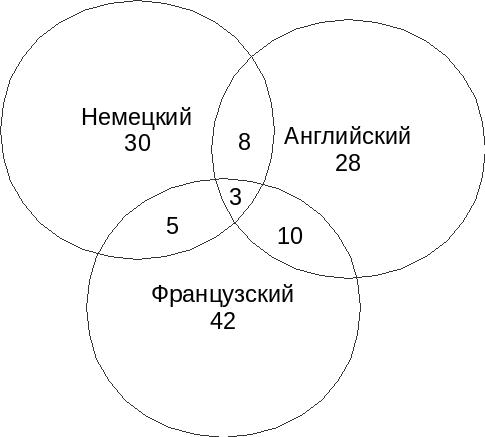
\includegraphics[width=.4\textwidth]{./pictures/1_23.png}
  \caption{Диаграмма Эйлера-Венна для задачи 1.23}
  \label{fig:123}
\end{figure}

Сначала найдём, сколько студентов знает хотя бы один язык.
Это есть мощность (количество элементов) объединения трёх множеств: Английский, Немецкий и Французский, которые обозначим первыми буквами.
Мощность объединения трёх множеств можно найти как сумму мощностей этих множеств, но, так как они пересекаются,
необходимо отнять мощности их пересечений и добавить пересечение всех трёх множеств, потому что его отняли дважды.
Имеем
\begin{equation*}
\begin{split}
|H \cup A \cup F| =
|H| + |A| + |F| - |H \cap A| - |A \cap F| - |H \cap F| + |H \cap A \cap F| = \\
= 30 + 42 + 28 - 5 - 8 - 10 + 3 = 80.
\end{split}
\end{equation*}

Все остальные студенты из ста не знают ни одного языка.
Их 
$$ 100 - 80 = 20.$$
